\documentclass{article}
\usepackage[a4paper, total={6in, 10in}]{geometry}

\usepackage[utf8]{inputenc}
\usepackage{graphicx}
\usepackage{amsmath, amssymb}
\usepackage{empheq}
\usepackage{showlabels}
\usepackage{graphicx}
\graphicspath{ {./img_formula/} }
\usepackage{float}  % In preamble

% Tiếng Việt
\usepackage[utf8]{vietnam}
% Thụt đầu dòng
\usepackage{indentfirst}
% Chia nhiều cột trên trang
\usepackage{multicol}
% List
\usepackage{enumitem}
% Table
\usepackage[thinlines]{easytable}
% multiple col
\usepackage{multicol}


\begin{document}

\author{}
\title{Basic Math for Physics}
\date{Mar/22/2025}

\maketitle
\tableofcontents
\newpage

\section{Quadratic Equation - Phương trình bậc 2}

Với phương trình $ax^2 + bx + c = 0 \ (a \neq 0)$. \par

Ta có $\Delta = b^2 - 4ac$. \par

\textbf{TH1.} $\Delta < 0$ phương trình vô nghiệm \par

\textbf{TH2.} $\Delta = 0$ phương trình có nghiệm kép $x_1 = x_2 = -\frac{b}{2ac}$ \par

\textbf{TH3.} $\Delta > 0$ phương trình có hai nghiệm phân biệt $x_{1;2} = \frac{-b\pm \sqrt{\Delta}}{2a}$

\section{Common Formulae of Algebra - Hằng đẳng thức đáng nhớ}
\begin{enumerate}[label=(\roman*)]
	\item $(a+b)^2 = a^2 + b^2 + 2ab$
	\item $(a-b)^2 = a^2 + b^2 - 2ab$
	\item $(a+b)(a-b) = a^2 - b^2$
	\item $(a+b)^3 = a^3 + b^3 + 3ab(a+b)$
	\item $(a-b)^3 = a^3 - b^3 - 3ab(a-b)$
	\item $(a+b)^2 - (a-b)^2 = 4ab$
	\item $(a+b)^2 + (a-b)^2 = 2(a^2 + b^2)$
	\item $a^3 - b^3 = (a-b)(a^2 + b^2 + ab)$
	\item $a^3 + b^3 = (a+b)(a^2 + b^2 - ab)$

	\item $(a+b+c)^2 = a^2 + b^2 + c^2 + 2ab + 2bc + 2ca$
	\item $(a-b-c)^2 = a^2 + b^2 + c^2 - 2ab + 2bc - 2ca$
	\item $(a+b-c)^2 = a^2 + b^2 + c^2 + 2ab - 2bc - 2ca$
	\item $(a+b+c)^3 = a^3 + b^3 + c^3 + 3(a+b)(b+c)(c+a)$
\end{enumerate}

\section{Arithmetic Progression - Tiến trình số học}
\begin{enumerate}[label=(\roman*)]
	
	\item $n^{th}$ term of arithmetic progression
	\begin{align*}
		a_n = a_0 + (n - 1)d
	\end{align*}
	$a_0 =$ First term, \\
	$n =$ Number of terms, \\
	$d =$ Common difference \\
	$ = (a_1 - a_0)$ or $(a_2 - a_1)$ or $(a_3 - a_2)$
	
	\item Sum of arithmetic progression
	\begin{align*}
		S_n = \frac{n}{2}[2a_0 + (n-1)d] = \frac{n}{2}[a_0 + a_n]
	\end{align*}
	$a_n =$ last term	
\end{enumerate}

\section{Geometric Progression - Tiến trình hình học}
Here $a = \text{first term}, r = \text{common ratio (tỷ lệ chung)}$
\begin{enumerate}[label=(\roman*)]
    \item Sum of $'n'$ terms of G.P
    \begin{align*}
        &S_n = \frac{a(1-r^n)}{1-r} \quad \text{if} \quad r < 1 \\
        &S_n = \frac{a(r^n - 1)}{r-1} \quad \text{if} \quad r > 1
    \end{align*}
    \item Sum of infinite terms of G.P
    \begin{align*}
        &S_{\infty} = \frac{a}{1-r} \quad \text{if} \quad r < 1 \\
        &S_{\infty} = \frac{a}{r-1} \quad \text{if} \quad r > 1
    \end{align*}
\end{enumerate}

\section{Trigonometry Angle}

\begin{figure}[H]
    \centering
    \caption{Length of chord}
    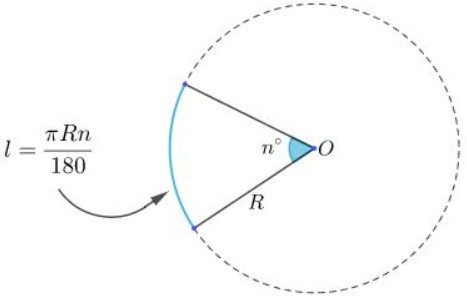
\includegraphics[width=0.4\textwidth]{chord_length.png}
\end{figure}

\begin{align*}
    &Angle(\theta) = \frac{Arc Length}{Radius} = \frac{L}{r} \\
    &(\text{formula true for radian only})
\end{align*}

\section{Trigonometry Ratio}
\begin{align*}
    &sin(\theta) = \frac{Perpendicular}{Hypotenuse} = \frac{p}{h} = \text{đi học} \\
    &cos(\theta) = \frac{Base}{Hypotenuse} = \frac{b}{h} = \text{không hư} \\
    &tan(\theta) = \frac{sin(\theta)}{cos(\theta)} = \frac{Perpendicular}{Base} = \frac{p}{b} = \text{đoàn kết} \\
    &cosec(\theta) = \frac{1}{sin(\theta)}; \qquad
    sec(\theta) = \frac{1}{cos(\theta)}; \qquad
    cot(\theta) = \frac{1}{tan(\theta)} = \frac{\cos(x)}{\sin(x)}
\end{align*}

\section{Trigonometry values of Larger Angles}
\begin{align*}
    &sin(180^o - \theta) = sin(\theta) \qquad sin(360^o - \theta) = -sin(\theta) \\
    &cos(180^o - \theta) = -cos(\theta) \qquad cos(360^o - \theta) = cos(\theta) \\
    &tan(180^o - \theta) = -tan(\theta) \qquad tan(360^o - \theta) = -tan(\theta) \\
    &sin(180^o + \theta) = -sin(\theta) \qquad sin(360n^o + \theta) = sin(\theta) \\
    &cos(180^o + \theta) = -cos(\theta) \qquad cos(360n^o + \theta) = cos(\theta) \\
    &tan(180^o + \theta) = tan(\theta) \qquad tan(360n^o + \theta) = tan(\theta)
\end{align*}

\section{Trigonometrical Indentities}
\begin{enumerate}[label=(\roman*)]
    \item $sin^2(\theta) + cos^2(\theta)= 1$
    \item $sec^2(\theta) - tan^2(\theta)= 1$
    \item $cosec^2(\theta) + cot^2(\theta)= 1$
\end{enumerate}

\section{Trigonometry Formulae}
\begin{align*}
    &sin(A+B) = sin(A)cos(B) + cos(A)sin(B) \\
    &sin(A-B) = sin(A)cos(B) - cos(A)sin(B) \\
    &cos(A+B) = cos(A)cos(B) - sin(A)sin(B) \\
    &cos(A-B) = cos(A)cos(B) + sin(A)sin(B) \\
    &tan(A+B) = \frac{tan(A)+tan(B)}{1-tan(A)tan(B)} \\
    &tan(A-B) = \frac{tan(A)-tan(B)}{1+tan(A)tan(B)} \\
    &sin(2\theta) = 2sin(\theta)cos(\theta) \\
    &cos(2\theta) = cos^2(\theta) - sin^2(\theta) = 2cos^2(\theta - 1) = 1 - 2sin^2(\theta) \\
    &tan(2\theta) = \frac{2tan(\theta)}{1-tan^2(\theta)}
\end{align*}

\section{Logarithm}
If $a^x= N$ then $log_a(N)=x$ \\
Conversion of natural log into common log:
\begin{align*}
    log_e(x) = ln(x) = 2.3026log_{10}(x)
\end{align*}

\section{Important formulae of logarithm}
\begin{enumerate}[label=(\roman*)]
    \item $log_{a}(m.n) = log_a(m) + log_a(n)$
    \item $log_a(m/n)=log_a(m)-log_a(n)$
    \item $log_a(m^n)=nlog_a(m)$
\end{enumerate}

\section{Differential Calculus}

\begingroup

\setlength{\tabcolsep}{10pt} % Default value: 6pt
\renewcommand{\arraystretch}{2} % Default value: 1

\begin{table}[!ht]
\centering
\begin{tabular}{|l|l|l|l|}
\hline
$y=x^n$         & $\frac{dy}{dx}=nx^{n-1}$              & $y=sin(x)$   & $\frac{dy}{dx}=cos(x)$          \\ \hline
$y=kx$          & $\frac{dy}{dx}=k\frac{dx}{dx}=k$      & $y=cos(x)$   & $\frac{dy}{dx}=-sin(x)$         \\ \hline
$y=k$           & $\frac{dy}{dx}=0$                     & $y=tan(x)$   & $\frac{dy}{dx}=sec^{2}(x)$      \\ \hline
$y=\frac{1}{x}$ & $\frac{dy}{dx}=-\frac{1}{x^2}$        & $y=coses(x)$ & $\frac{dy}{dx}=-cot(x)cosec(x)$ \\ \hline
$y=\sqrt{x}$    & $\frac{dy}{dx}=\frac{1}{2\sqrt{x}}$   & $y=sec(x)$   & $\frac{dy}{dx}=sec(x)tan(x)$    \\ \hline
$y=ln(x)$       & $\frac{dy}{dx}=\frac{1}{x}$           & $y=cot(x)$   & $\frac{dy}{dx}=-cosec^{2}(x)$   \\ \hline
$y=log_{a}(x)$  & $\frac{dy}{dx}=\frac{1}{x}log_{a}(e)$ &              &                                 \\ \hline
$y=e^{x}$       & $\frac{dy}{dx}=e^{x}$                 &              &                                 \\ \hline
$y=a^{x}$       & $\frac{dy}{dx}=a^{x}log_{e}(a)$       &              &                                 \\ \hline
\end{tabular}
\end{table}

\begin{table}[!ht]
\centering
\begin{tabular}{|l|l|l|l|}
\hline
$(u+v)'=u'+v'$                                   & $(u-v)'=u'-v'$            & $(u.v)'=u'v+v'u$                            & $(\frac{u}{v})'=\frac{u'.v-v'.u}{v^2}$ \\ \hline
$(e^u)’=u’.e^u$                                  & $ln(u)’=\frac{u’}{u}$     & $(u^{\alpha})’=\alpha . u^{\alpha -1} . u’$ & $(\sqrt{u})’=\frac{u’}{2\sqrt{u}}$     \\ \hline
$(\sqrt[n]{u})’ = \frac{u’}{n\sqrt[n]{u^{n-1}}}$ & $(\sin(u))’ = u’.\cos(u)$ & $(\cos(u))’ = -u’.\sin(u)$                  & $(a^u)’=u’.a^u.ln(a)$                  \\ \hline
$(log_{a}(u))’ = \frac{u’}{u.ln(a)}$             &                           &                                             &                                        \\ \hline
\end{tabular}
\end{table}

\begin{align*}
    &(\tan(u))' = \frac{u'}{\cos^2(u)} \\
    &(\cot(u))' = -\frac{u'}{\sin^2(u)} \\
    &\Big[(x^m)^n\Big]' = (m\geq n) \quad ? \quad m(m-1)(m-2)(m-n+1)x^{m-n} : 0 \\
    &(\log_{a}(x))^n = (-1)^{n-1}. \frac{(n-1)!}{\ln(a)}\frac{1}{x^n} \\
    &(\ln(x))^n = (-1)^{n-1}.(n-1)!.x^{-n} \\
    &(e^{kx})^n = k^n.e^{kx} \\
    &(a^x)^n = (\ln(a))^n.a^x \\
    &(\sin(ax))^n = a^n.\sin(ax + n.\pi/2) \\
    &(\cos(ax))^n = a^n.\cos(ax + n.\pi/2) \\
    &\Big(\frac{1}{ax+b}\Big)^{n} = (-1)^{n}.a^n.n!.\frac{1}{(ax+b)^{n+1}} \\
    &(\arcsin(x))' = \frac{1}{\sqrt{1-x^2}} \\
    &(\arccos(x))' = \frac{-1}{\sqrt{1-x^2}} \\
    &(\arctan(x))' = \frac{1}{1 + x^2}
\end{align*}

\noindent Chain rule
\begin{align*}
    \Bigg[f\Big(g(x)\Big)\Bigg]'=f'\Big(g(x)\Big).g'(x)
\end{align*}

\endgroup

\newpage
\section{Integral Calculus}

\begingroup

\setlength{\tabcolsep}{10pt} % Default value: 6pt
\renewcommand{\arraystretch}{2} % Default value: 1

\begin{table}[!ht]
\centering
\begin{tabular}{|l|l|l|l|}
\hline
$y=x^n$         & $\int x^ndx = \frac{x^{n+1}}{n+1} + c$   & $y=sin(x)$         & $\int sin(x)dx = -cos(x)$           \\ \hline
$y=k$           & $\int kdx = kx + c$                      & $y=cos(x)$         & $\int cos(x)dx=sin(x)$              \\ \hline
$y=1$           & $\int dx = x + c$                        & $y=sec^2(x)$       & $\int sec^2(x)dx = tan(x)$          \\ \hline
$y=\frac{1}{x}$ & $\int \frac{1}{x}dx = ln(x) + c$         & $y=sec(x)tan(x)$   & $\int sec(x)tan(x)dx = sec(x)$      \\ \hline
$y=e^{x}$       & $\int e^{x}dx = e^{x} + c$               & $y=cosec^2(x)$     & $\int cosec^2(x)dx = -cot(x)$       \\ \hline
$y=a^{x}$       & $\int a^x dx = \frac{a^x}{log_e(a)} + c$ & $y=cosec(x)cot(x)$ & $\int cosec(x)cot(x)dx = -cosec(x)$ \\ \hline
\end{tabular}
\end{table}

\endgroup


\section{Circumferences}

\begin{multicols}{2}
\begin{enumerate}
    \item Circumderence of circle: $C = 2\pi R$
    \item Circumderence of triangle: $P = a + b + c$
\end{enumerate}

\end{multicols}


\section{Formulae for Area and Volume}

\begin{multicols}{2}

\begin{enumerate}
    \item Area of square $=(side)^2$
    \item Area of rectangle $=length \times length$
    \item Area of triangle $=\frac{1}{2}\times base\times height$ 
    \item Area of equilateral triangle $=\frac{\sqrt{3}}{4}a^2$
    \item Are enclosed by a circle $=\pi r^2$
    \item Surface area of sphere $=4\pi r^2$
    \item Surface area of cube $=6L^2$
    \item Surface area of cuboid \\ $=2[L\times b + b\times h + h\times L]$
    \item Area of curved surface of cylinder $=2\pi rl$
    \item Volume of cube $=L^3$
    \item Volume of cuboid $=L\times b\times h$
    \item Volume of sphere $=\frac{4}{3}\pi r^3$
    \item Volume of cylinder $=\pi r^3 l$
    \item Volume of cone $=\frac{1}{2}\pi r^2 h$
\end{enumerate}

\end{multicols}


\end{document}